\documentclass[usenatbib]{mn2e} 
\usepackage{url}
\usepackage{amsmath} 
\usepackage{amssymb} 
\usepackage{graphics}
\usepackage{epsfig}  
\def\be{\begin{equation}}
\def\ee{\end{equation}}
\def\ba{\begin{eqnarray}}
\def\ea{\end{eqnarray}}

% To highlight comments 
\usepackage{color}
\definecolor{red}{rgb}{1,0.0,0.0}
\newcommand{\red}{\color{red}}

\usepackage[normalem]{ulem}
\definecolor{darkgreen}{rgb}{0.0,0.5,0.0}
\newcommand{\SRK}[1]{\textcolor{darkgreen}{\bf SRK: \textit{#1}}}
\newcommand{\SRKED}[1]{\textcolor{darkgreen}{\bf #1}}

\newcommand{\LCDM}{$\Lambda$CDM~}
\newcommand{\beq}{\begin{eqnarray}}  
\newcommand{\eeq}{\end{eqnarray}}  
\newcommand{\zz}{$z\sim 3$}  
\newcommand{\apj}{ApJ}  
\newcommand{\apjs}{ApJS}  
\newcommand{\apjl}{ApJL}  
\newcommand{\aj}{AJ}  
\newcommand{\mnras}{MNRAS}  
\newcommand{\mnrassub}{MNRAS accepted}  
\newcommand{\aap}{A\&A}  
\newcommand{\aaps}{A\&AS}  
\newcommand{\araa}{ARA\&A}  
\newcommand{\nat}{Nature}  
\newcommand{\physrep}{PhR}
\newcommand{\pasp}{PASP}    
\newcommand{\pasj}{PASJ}    
\newcommand{\avg}[1]{\langle{#1}\rangle}  
\newcommand{\ly}{{\ifmmode{{\rm Ly}\alpha}\else{Ly$\alpha$}\fi}}
\newcommand{\Mpc}{{\ifmmode{{\rm Mpc}}\else{Mpc }\fi}}  
\newcommand{\hMpc}{{\ifmmode{h^{-1}{\rm Mpc}}\else{$h^{-1}$Mpc }\fi}}  
\newcommand{\hGpc}{{\ifmmode{h^{-1}{\rm Gpc}}\else{$h^{-1}$Gpc }\fi}}  
\newcommand{\hmpc}{{\ifmmode{h^{-1}{\rm Mpc}}\else{$h^{-1}$Mpc }\fi}}  
\newcommand{\hkpc}{{\ifmmode{h^{-1}{\rm kpc}}\else{$h^{-1}$kpc }\fi}}  
\newcommand{\hMsun}{{\ifmmode{h^{-1}{\rm {M_{\odot}}}}\else{$h^{-1}{\rm{M_{\odot}}}$}\fi}}  
\newcommand{\hmsun}{{\ifmmode{h^{-1}{\rm {M_{\odot}}}}\else{$h^{-1}{\rm{M_{\odot}}}$}\fi}}  
\newcommand{\Msun}{{\ifmmode{{\rm {M_{\odot}}}}\else{${\rm{M_{\odot}}}$}\fi}}  
\newcommand{\msun}{{\ifmmode{{\rm {M_{\odot}}}}\else{${\rm{M_{\odot}}}$}\fi}}  
\newcommand{\lya}{{Lyman-$\alpha$ }}
\newcommand{\clara}{{\texttt{CLARA}}~}
\newcommand{\rand}{{\ifmmode{{\mathcal{R}}}\else{${\mathcal{R}}$ }\fi}}  
\begin{document}

\title[The baryonic LG in SAMs]{The baryonic properties of the Local Group: a semi-analytic perspective}
\author[Sanes et al.]{
\parbox[t]{\textwidth}{\raggedright 
  Sergio Sanes \thanks{email}$^1$, 
  Jaime E. Forero-Romero$^2$,
  Juan C. Munoz-Cuartas$^2$,
  Luis F. \\Quiroga-Pelaez$^1$,
  Jorge I. Zuluaga$^1$,
  Stefan Gottl\"ober$^2$,
  Yehuda Hoffman$^3$,\\  
  Gustavo Yepes$^4$}.
\vspace*{6pt}\\
$^1$Universidad de Antioquia\\
$^2$Leibniz-Institut f\"ur Astrophysik Potsdam (AIP), An der Sternwarte 16, 14482 Potsdam, Germany\\ 
$^3$Racah Institute of Physics, Hebrew University, Jerusalem 91904, 
 Israel\\ 
$^4$Grupo de Astrof\'{\i}sica, Universidad Aut\'onoma de Madrid,   Madrid
E-28049, Spain\\
}
\maketitle

\begin{abstract}

\end{abstract}
\begin{keywords}
galaxies: evolution - galaxies: formation -
galaxies: high-redshift - methods: N-body simulations
\end{keywords}

% KEY IDEAS
% IT IS NOT NECCESARY TO CHECJ IF THE SAMPLE IS BIASED, JAIME  ALREADY DID IT.
% WE DO NOT NEED TO SEARCH FOR SELECTION PARAMETERS TO FIND MW AS OTHER PAPERS (EJ. De Rossi et al)




\section{Introduction}
\label{sec:introduction}


\section{semi-analytics and the simulations}
\subsection{The Semi-Analytic Method}
\label{sec:sams}
We use the semi-analytic code of galaxy formation Galacticus \citep{2010arXiv1008.1786B}, designed to  by means of the hierarchical  merging
 history of a dark matter halo, estimate the properties of the galaxies hosted in it at any instant of its evolution.  

The code can include any model of physical process, starting from the generation of random dark matter density distributions to calculate stellar population 
properties while implementing accretion of gas, cooling, stellar and supernovae feedback. Depending of the needs, it is capable of generate its 
own Monte Carlo merger trees or just read  merger trees provided by cosmological simulations as we did taking advantage of the 
CLUES\footnote{Constrained Local UniversE Simulations} project\footnote{\url{http://www.clues-project.org/}}  simulations. The 
remaining of this section is dedicated to explain how Galacticus model the key astrophysical processes regarding our research.

Halos can increase their mass a consequence of mergers or accretion from the interstellar medium. In our selected model the accretion rate of gas
 from the interstellar medium into a dark matter halo is modeled by assuming that the amount of accreted baryonic  matter is directly related to the 
amount of accreted dark mass by the universal baryonic fraction  $\Omega_b/\Omega_M$. This can be expressed as
\begin{equation}
 \dot{M}_{\text{accre}}=
\begin{cases}
 (\Omega_b/\Omega_M)\dot{M}_{\text{halo}},\quad \text{if} \quad V_{\text{virial}}>V_{\text{reioniz}}\\
\qquad \qquad \qquad \qquad \text{or} \quad z>z_{\text{reioniz}}\\
0, \text{otherwise}
\end{cases}
\end{equation}
where the effects of reionization are taken in to account by  imposing the condition that no gas can be accreted at  redshifts $z$ higher than the one of 
reionization $z_{\text{reioniz}}$ or if the virial velocity $V_{\text{virial}}$ is less than the one of reionization $V_{\text{reioniz}}$. 
In case of a merger the whole mass of the satellite $M_{\text{satel}}$ and central $M_{\text{central}}$ goes to the bulge component of the central galaxy
when the satellite-to-central mass ratio $M_{\text{central}}/M_{\text{satel}}$ is above the major-to-minor merger fraction $\eta$, meaning  a major merger.
If a minor merger occurs the mass of the central galaxy does not moves, the stars of the satellite goes to the bulge of the central and according to a 
a free parameter of the model the gas mass $M_{\text{satel.,gas}}$ can be moved to the disk or to the bulge.

The cooling rate according to \cite{1991ApJ...379...52W} is given by
\begin{equation}
 \dot{M}_{cool}=4\pi r^2_{\text{cool}} \rho (r_{\text{cool}}) \dot{r}_{\text{cool}}
\end{equation}
where  $\rho(r)$ is the density profile of the hot halo and the cooling raduis $\dot{r}_{\text{cool}}$ is calculted by seeking the radius at which the 
time available for cooling equals the cooling time $t_{\text{cool}}$. 

Then the cooled gas is transformed into stars according to the star formation rate of the spheroid and disk components of the galaxy which are assumed to be fixed and of the form 
$\phi=M_{\text{gas}}/\tau_{\star}$, where $M_{\text{gas}}$ is the amount cold gas and 
\begin{equation}
 \tau_{\star} = \epsilon^{-1}_{\star}\tau_{\text{dyn}}\left( \frac{V}{200\text{km/s}}\right)^{\alpha_\star}
\end{equation}
is the star formation time scale (a similar expression of the one of \cite{2005MNRAS.356.1191B}) where $\tau_{\text{dyn}}$ is the dynamical time defined as
 $\tau_{\text{dyn}}=R_{\text{virial}}/V_{\text{circ}}$,  $R_{\text{virial}}$ and $V_{\text{circ}}$ are the characteristic radius and velocity respectively, 
the free parameter $\epsilon_{\star}$ is the star formation efficiency  and  $\alpha_\star$ is a free parameter as well.

We used the simplest method to model the increase of stellar mass. We relate the star formation rate $\phi$  to the stellar mass 
rate $\dot{M}_{\star}$ by a means of a constant rate of decrease of fuel mass as
\begin{equation}
 \dot{M}_{\star}=(1-R)\phi,
\end{equation}
where $R$ is the instantaneous recycled fraction. The rate of the metal content of the fuel changes as the star formation rate, the yield $p$ and $R$  according to
\begin{equation}  
 \dot{M}_{\text{fuel},Z}=-(1-R)Z_{\text{fuel}}\phi+p\phi,
\end{equation}
while the rate of change the metal content of the stars $\dot{M}_{\star, Z}$ follows from the fuel metallicity $Z_{\text{fuel}}$. We have used the Salpeter initial
 mass function \citep{1955ApJ...121..161S} to estimate the values of $R$ and $p$. Another important process we have aboarded is the supernovae feedback driven outflow that is 
modeled for the disks and the bulge of the galaxies through a power law relation and it is assumed to be  proportional to the rate of energy pumped in to the
 gas by the stellar populations. The rate of change of the mass expulsed by supernovae is given by
\begin{equation}
 \dot{M}_{\text{outflow}}=\left( \frac{V_{\text{outflow}}}{V} \right)^{\alpha_{\text{outflow}}}\frac{\dot{E}}{E_{\text{canonical}}}, \label{eq:supernovae}
\end{equation}
where  $V_{\text{outflow}}$ is the velocity of the ejected outflow mass due to supernovae, $V$ is the characteristic velocity,  $\dot{E}$ is the rate of change of 
the energy transmitted to the gas by stars and $E_{\text{canonical}}$ is the total energy transmitted by a stellar population normalized to $1M_{\odot}$.


\subsection{Contrained N-body simulations and Merger Trees}
\label{sec:simulations}
In this section we briefly describe the information of the CLUES simulations relevant to our research, the procedure of constraining cosmological simulations and 
construction of merger trees. 

We have selected the three available realizations for the WMAP5 cosmology of the CLUES \citep{2010arXiv1005.2687G}
which is aimed to provide constrained cosmological simulations recreating the Local Universe. As the CLUES simulations are intended to recreate the Local Universe
 they contain a set of dark matter halos candidates that should host galaxies with properties quite similar to those of the ones of the Local neighborhood galaxies
 including the Milky Way and Andromeda. We will give special attention to those halos candidates that should contain the Milky Way and Andromeda which from now we 
will call a Local Group candidates. Each of these simulations includes $1024^3$ particles with a mass of $m_{p}=1.89\times 10^{7}$\hMsun inside a box of side length $64$\hMpc  that provides an amount of more than
 $5\times 10^4$ dark matter merger trees \citep{2011arXiv1107.0017F}. The cosmological parameters are consistent with the WMAP5 cosmology in \cite{2009ApJS..180..330K}
 with a density $\Omega_{m}=0.279$, a cosmological constant $\Omega_{\Lambda} = 0.721$, a dimensionless Hubble parameter $h=0.70$, a spectral index of primordial
 density perturbations $n=0.96$, a normalization $\sigma_{8}=0.817$.  The code used to perform the simulations is the Tree-PM MPI N-body code Gadget2 \citep{2005MNRAS.364.1105S}. 
 From the set of three  realizations for the WMAP5 cosmology   we selected the set of merger trees whose dark matter halos at $z=0$ are in the mass 
range $11.0<\log_{10} M_{vir}/M_{\odot}<13.0$ and make an special emphasys in the subrange $11.5<\log_{10} M_{vir}/M_{\odot}<12.5$ to study MW and M31-type galaxies.  



The standard procedure of building by means of simulations a Local Universe able to recreate the main features of the observed is to constrain the initial conditions
to observations. For the CLUES simulations it was used the \cite{1991ApJ...380L...5H} algorithm  to constrain the Gaussian random fields to observational data. Due to
its very small changes in time, the velocity field played a crucial roll in constraining the initial conditions. To set up the velocity constrains the MARK
  III \citep{1997ApJS..109..333W}, SBF \citep{2001ApJ...546..681T} and the Karachentsev \citep{2004AJ....127.2031K} catalogs were used \citep{2011arXiv1107.0017F},
for more details of the constraining procedure go to \cite{2010arXiv1005.2687G}. As the constrains can only affect the large and meso scales, it was necessary to 
perform a large amount of low resolution simulations. Only three of all the simulations were had success in recreating under a certain accurately the properties
of the dark matter distribution.


The catalogue of dark matter halo merger trees used is the one of \cite{2011arXiv1107.0017F}. To identify halos it was used a FOF (Friends-of-Friends) algorithm 
in 80 snapshots corresponding to an interval of about 13Grys between $0<z<7$, where it was not included any substructure information. It was used a linking length of 
$b=0.17$ times the mean inter particle separation and the minimum resolved halo masses are of $M_{\text{min}}=3.78\times 10^8 \hMsun$. The procedure used to build the
 merger trees is the standard. Starting from the snapshot at $z=0$, the particles bind to a particular  halo of the catalogue are scanned in the first snapshot $z>0$ 
and if there it is found any halo with more than thirteen particles then then this halo is called to be a progenitor of the former. The process is repeated over the whole
catalogue at $z=0$ and continued until the highest $z$. For more details about the halo identification and merger tree construction go to \cite{2011arXiv1107.0017F}.
 

 To perform our simulations, it was only used the information relating the masses of the satellites and central dark matter halos over the different snapshots to its 
progenitors, the detailed information of how are built the input dark matter halo merger trees for Galacticus go to \cite{2010arXiv1008.1786B}.

\section{The observational prorperties of MW and M31}  
\label{sec:discussion}  

In this section we present the values for the parameters we have chosen to define the MW and M31: disk stellar mass, disk gaseous mass and bulge stellar mass.

{\bf Disk stellar mass}. The principal approach to estimate the stellar mass in the disk of our galaxy is dynamical modelling. The work of \cite{Klypin2002} uses a parametric model
 that does not distinguish between the cold (gas) component and the stars, their results for galaxy models that allow for exchange of angular momentum locate the total baryonic mass
 of the disk between $5-6\times 10^{10}$\Msun for the MW and $7-9\times 10$\Msun for M31. Later \cite{Widrow2005} use N-body realizations of self-consisten, equilibrium distributions 
of the dark matter and stellar compoents to address the same problem. Their models fit with good match to the observational data have stellar masses of $3.3-4.5\times 10^{10}$\Msun for 
the Milky Way and $7-10\times 10^{10}$ for andromeda. \citep{Geehan2006} modeled the Andromeda strem using analytic bulge-disc-halo for M31, finding the best agreement for a disk 
mass of $8.4\times 10^{10}$\Msun. In this work we take $3.3-4.5\times 10^{10}$\Msun for the Milky Way and $7-10\times 10^{10}$ for M31.  

{\bf Bulge stellar mass}. \cite{Klypin2002} constrain the MW bulge stellar masss $1-1.2\times 10^{10}$ \Msun while for M31 $1.9-2.4\times 10^{10}$, for the same galaxy 
\citep{Geehan2006} find a bulge mass of $3.3\times 10^{10}$\Msun. The MW analytical model of model \citep{Dehnen1998} finds a range of different values with average 
$\sim 0.5 10^{10}$\Msun. In this work we pick $0.5-1.2 \times 10^{10}$\Msun for the MW and $1.9-3.3\times 10^{10}$\Msun for M31.

{\bf Disk Gaseous mass}. The abundance of gas in the Milky Way has been constrained through chemical evolution models. The set of observational constraints on these models most 
notably include the gas and star formation rate (SFR) profiles. The relevant observational data was compiled in \citep{Boissier99} using from the original work in 
\cite{Kulkarni87,Dame93}, with a values of $6.0-8.0 \times 10^{9}$\Msun, an update implementation of this chemical evolution model by \citep{Yin09} uses the same observations. 
In the case of M31 the best observational constraints come from the observations by \citep{Cram80} with the integrated mass of neutral gas corrected by \citep{Dame93}, yielding a 
value of $5.2\times 10^{9}$\Msun, there is a systematic observational uncertainty of $5\%$ originally quoted in \citep{Cram80}, but due to oppacity effects of the HI \citep{Braun92}
 the total value of gas can increase by a $19\%$. Therefore we keep a value of $5.0-6.0\times 10^{9}$ for the mass of gas in the M31 disk and $6.0-8.0\times 10^{9}$\Msun for the
 Milky Way. 


\section{The Method}
\label{sec:method}


\subsection{Numerical Procedures}
\label{sec:method:numericals}
\begin{table*}\tiny
\centering
\resizebox{7in}{!} {
\begin{tabular}{|l|l|l|l|l|l|l|l|l|}
\hline
\hline
Model  &  $z_{reioniz}$ &  $M_{\text{satel.,gas}}\to$  & $\eta$ & $P(\lambda)$  &  $\mu_\lambda$
 & $\sigma_\lambda$  & $\alpha_{\text{disk,outflow}}$ & $\epsilon_{\text{disk},\star}$ \\
\hline
\hline
%\\[0pt]
R1 & 9.0 &  bulge & 0.3 &Bett 2007 & &  & 2.0 & 0.01 \\
%run-v2 & 7.0 &  bulge & 0.3 &Lognormal & 0.03687 & 0.2216 & 2.0 & 0.01 \\
R2 & 7.0 &  bulge & 0.3 &Lognormal & 0.031 & 0.57 & 2.0 & 0.01 \\
R3 & 7.0 &  disk & 0.3 &Lognormal & 0.031  & 0.57 & 2.0 & 0.01 \\
\hline
E1 & 7.0 &  disk & 0.3 &Lognormal & 0.031 & 0.57 & 2.0 & 0.02 \\
E2 & 7.0 &  disk & 0.3 &Lognormal & 0.031 & 0.57 & 2.0 & 0.035 \\
E3 & 7.0 &  disk & 0.3 &Lognormal & 0.031 & 0.57 & 2.0 & 0.05 \\
E4 & 7.0 &  disk & 0.3 &Lognormal & 0.031 & 0.57 & 2.0 & 0.075 \\
E5 & 7.0 &  disk & 0.3 &Lognormal & 0.031 & 0.57 & 2.0 & 0.1 \\
\hline
A1 & 7.0 &  disk & 0.3 &Lognormal & 0.031 & 0.57 & 1.5 & 0.01 \\
A2 & 7.0 &  disk & 0.3 &Lognormal & 0.031 & 0.57 & 2.5 & 0.01 \\
A3 & 7.0 &  disk & 0.3 &Lognormal & 0.031 & 0.57 & 3.0 & 0.01 \\
\hline
D1 & 7.0 &  disk & 0.2 &Lognormal & 0.031 & 0.57 & 2.0 & 0.01 \\
D2 & 7.0 &  disk & 0.4 &Lognormal & 0.031 & 0.57 & 2.0 & 0.01 \\
\hline
B1 & 7.0 &  bulge & 0.2 &Lognormal & 0.031 & 0.57 & 2.0 & 0.01 \\
B2 & 7.0 &  bulge & 0.4 &Lognormal & 0.031 & 0.57 & 2.0 & 0.01 \\
\hline
\hline
\end{tabular}
}
\caption{Set of four experiments intended to model the galaxies hosted in  halos of mass range of $11.0<log_{10} M_{\text{DM}}<13.0$.\label{tab:runs}}
\end{table*}
To achieve our goals we have used the semi-analytic code Galacticus v0.0.1 to perform semi-analytical simulations of different models to study the $z=0$  
properties of the simulated galaxies. The amount of halos in our selected mass range in section \ref{sec:simulations}) is above $9000$/box, then, accounting 
for a total of almost $30000$ merger trees when the three boxes are included. In this section we investigate  how sensitive could be the properties of the 
simulated  galaxies  to the variations of several parameters we pretent to study. To do this, we have simulated a set of models with parameters as shown Table 
\ref{tab:runs} where to be in agreement to the data we have settled the respective cosmology to WMAP5 and any other not mentioned parameters are settled to the
 code's default values (To see in detail the parameters and their values go to \cite{2010arXiv1008.1786B}). From the  simulated models of Table \ref{tab:runs}
 we have defined three benchmarks,  the first is R1 which is performed with a spin parameter distribution according to the one of \cite{2007MNRAS.376..215B}.
 For he two other simulated models R2 and R3,  we have settled the distribution of the spin parameter to a Lognormal distribution  with a mean 
 $\mu_{\lambda}=0.03687$ and dispersion $\sigma_{\lambda}=0.2216$ according to the work of \cite{2011MNRAS.411..584M} but in  R2 the gas of satellites after 
a minor merger goes to the bulge of the central galaxy and in the R3 the gas goes to the disk of the central galaxy. All the remaining models are settled to a
 Lognormal distribution with a mean $\mu_{\lambda}=0.03687$ and dispersion $\sigma_{\lambda}=0.2216$ as well. We have developed a set of four experiments 
intended to study how are affected the stellar-to-dark matter ratio, gas-to-total mass ratio and bulge-to-total mass ratio by the variation of  
$\alpha_{\text{outflow}}$, $\epsilon_\star$ for the disk component of the galaxies, $\eta$ and where does $M_{\text{satel.,gas}}$ goes after a minor merger.

As discribed in Table \ref{tab:runs}, in the set of E-labeled models, from our the selected halo population we have modeled galaxies  with 
$\epsilon_{disk,\star}=0.01, 0.02, 0.035, 0.05,0.075$ and $0.1$; In the A-labeled models, we selected the four values 1.5, 2.0, 2.5 and 3.0 for the 
$\alpha_{\text{disk,outflow}}$ parameter; In the D and B-labeled models we performed simulations to search wether there is any 
correlation between the studyed properties and the parameter $M_{\text{satel.,gas}}\to$ when it is settled to the disk and to the bulge, so, as we have a special
 interested in obtaining disk-type galaxies, for the most of the models  of Table \ref{tab:runs} we have settled $M_{\text{satel.,gas}}\to$ to the disk. In the
 two other experimets we set $M_{\text{satel.,gas}}\to$ to the disk and bulge while $\eta$ is settled to 0.2,0.3 and 0.4.


% We simulated the population of halos defined in Section \ref{sec:method:numericals}  under the  models with parameters  shown in Table \ref{tab:runs}; All other
%  parameters are settled to the code's default values (see \cite{2010arXiv1008.1786B}).
%
%  The models in Table \ref{tab:runs} are divided into four groups of experimets where we 
% have changed  the values of a certain group of parameters and criteria we belive can modify the resulting properties of a galaxy at $z=0$. 
%The parameters we have 
% selected to carry on our research are the star formation disk efficiency $\epsilon_{\text{disk},\star}$, the supernovae disk outflow exponent $\alpha_{\text{disk,outflow}}$, the
% major-to-minor merger fraction $\eta$ and the criterium $M_{\text{satel.,gas}}\to$ of where does the gas of a satellite  goes after a minor merger. 
%
% to see how much changes the amount of  LG-type galaxies when 
% 
 %(from now $\alpha_{\text{disk, outflow}}$, $\epsilon_{\text{disk,}\star}$)
\subsection{Searching LG-type Galaxies}
\label{sec:method:finding-lg}
Our investigation of the LG can be divided into two main parts. The first is intended to study  for the  different models in Table \ref{tab:runs}, the formation
 of MW  and M31-type galaxies given a catalogue of dark matter merger trees; In the second one, we study how peculiar are the LG candidates provided from the 
CLUES simulations in terms of the similarity of their properties compared to the observed ones.

To study the similarity between the observed and the simulated galaxy we make use of relative errors. Let an observed galaxy $\rho_{obs}(p_{obs,1}, \dots ,p_{obs,n})$ 
be characterized by an amount of $n$ observed properties $p_{obs,i}$, a simulated galaxy $R_{sim}(r_{sim,1}, \dots,r_{sim,n})$ characterized by the same amount
 of  estimated properties $r_{sim,i}$. The relative error between each observated property and the modelled is $\epsilon_i=|P_{obs,i}-R_{sim,i}|/|P_{obs,i}|$. Then,
we would use the addition of all the relative errors of all the properties
\begin{equation}
 \Delta \varepsilon = \epsilon_i+\dots+\epsilon_n.\label{eq:relative_error}
\end{equation}
% To study the similarity of a galaxy to any other, we define the $\chi^2$-type metric estimator
% \begin{equation}
%  \chi=\sum_i \left[ \frac{p_{i,sim} - p_{i,obs}}{p_{i,obs}}\right]^2, \label{eq:chi-crit}
% \end{equation}
% where we are compared the calculated properties  $p_{i,sim}$ against the current observational estimations $p_{i,obs}$ of any galaxy.
% To find how likely are the simulated galaxies of the models of Table \ref{tab:runs} to the LG, we have selected five different properties and compared the modeled 
% properties to the observed ones presented in Table \ref{tab:lg-observations}. According to the above definition of $\chi$, the closer the values of the compared
% properties, the lowest the value of $\chi$. A value of $\chi=0$ between two galaxies means that are definitly is equal to each other. We also defined a second 
% estimator $\gamma$ to study how biased can be the $\chi$ estimator. This second estimator is defined as
% \begin{align}
%  \gamma=&\sum_i \delta (p_{i,sim}, p_{i,obs})\\
% \delta (p_{i,sim}, p_{i,obs})=&
% \begin{cases}
% 1, &\left| \frac{p_{i,sim} - p_{i,obs}}{p_{i,obs}} \right| \le 0.15 \\
% 0, &\left| \frac{p_{i,sim} - p_{i,obs}}{p_{i,obs}} \right|>0.15.
% \end{cases}
% \end{align}
% Below a relative error of $15\%$, $\gamma$ accounts the number of properties that are close to the ones of the studyed galaxy, in our particular case, the Milky Way and 
% Andromeda.
                                                                                                                                                                                                                                                                                                                                                                                                                                                                                                                                                                                             

To study how much changes the abundance of LG-type galaxies for each of the performed models, we accounted the amount of galaxies $N(\Delta \varepsilon)$
similar to the MW and M31 under a ranges of calculated total relative error  $\Delta \varepsilon$ as defined in equation \ref{eq:relative_error}. We selected 
three the lowest values of $\Delta \varepsilon$ (0.08, 0.16 and 0.24) and studyed its variations of $N(\Delta \varepsilon)$ as a function of the studyed 
parameters in order find lights about wether there is any set values for our selected set of parameter that $1)$ increases the abundace of disk galaxies $2)$
increases the amount of MW and M31-type of galaxies.
 
\begin{table}
\centering
\begin{tabular}{|l|l|l|l|l|}
\hline
\hline
 Property &  MW &  Ref. & M31 & Ref.\\
\hline
$M_{disk,\star}[10^{10}M_{\odot}]$ & $3.0 $ &  $(1)$ & $7.2$ & $(2)$ \\
$M_{disk,gas}[10^{10}M_{\odot}]$ & $0.7$ &  $(3)$ & $0.6$ &  $(4)$ \\
$M_{bulge,\star}[10^{10}M_{\odot}]$ & $1-2$ & $(3)$ & $3.2$ &  $(2)$ \\
$V_{circ}[\text{Km/s}]$ & $238$ &  $(5)$ & $275\pm 5$ & $(6)$ \\
%& $220$ & $(7)$ &   &  \\
%$r_d[\text{Kpc}]$ & $2.38$ & $(5)$  & $5.48$ & $(3)$  \\
 %&  $3.7\pm 1$ &  & ...  \\
\hline
\hline
\end{tabular}
\caption{Observational estimations for different properties of the LG, where$(1)$\citet{2001ApJ...555..393Z},
$(2)$ \citet{2006MNRAS.366..996G}, $(3)$\citet{2009A&A...505..497Y}, $(4)$ \citet{2006A&A...453..459N}, $(5)$\citet{2005MNRAS.364..433B}, 
$(6)$\citet{2008MNRAS.389.1911S}.
}
\label{tab:lg-observations}
\end{table}

\subsection{Modeling the LG candidates}
\label{sec:modeling-lg}
We proceded to model semi-analyticaly the  pairs of LG candidates  available from the three WMAP5 boxes of CLUES.

Two experiments were performed. Given the preliminar results of sections \ref{sec:method:numericals} and \ref{sec:method:finding-lg}, 
we settled the space parameter of the two experiments to a WMAP5 cosmology and $M_{\text{satel.,gas}}\to$ to the disk component of the galaxy.
The first experiment was intended to recreate the experiment of the A-labeled models of Table \ref{tab:runs}, so, we simulated the LG halo candidates for different
values of $\alpha_{\text{disk,outflow}}$ ranging from 1.5  to 3.0 in steps of 0.075. For each of the values of $\alpha_{\text{disk,outflow}}$, we repeated
the simulation 100 times and calculated the medians of the properties of MW and M31; 
In the second experiment, we recreate the experiement of the E-labeled models.  We simulated the LG candidates through 20 different models of 
$\epsilon_{\text{disk},\star}$, starting from 0.005 in steps of 0.005 to 0.1, repeated the simulation 100 times for each value of 
$\epsilon_{\text{disk},\star}$ and calculated the medians of the properties as well. Finally  it was also applied the same searching criterium of equation
\ref{eq:relative_error} to look for similarities between the LG modeled pairs and the observed M31 and MW.
\section{Results}
\subsection{Test on Galacticus}
\begin{figure}
\centering
 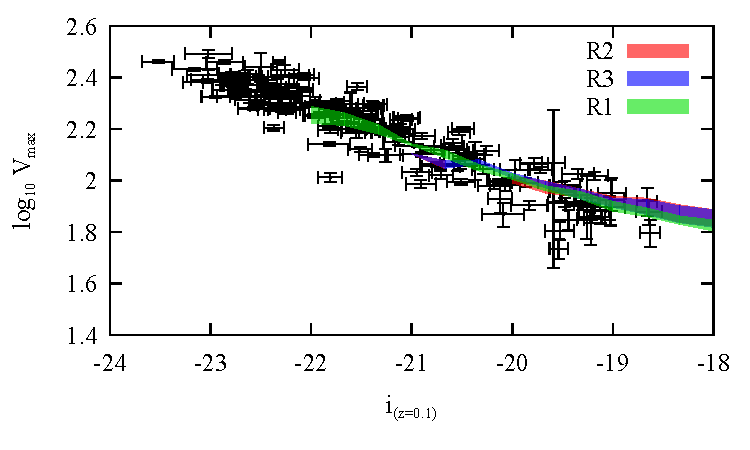
\includegraphics[scale=0.68]{figures/tests/T_F-disk-velmax.pdf}
\caption{ Tully fischer relation. The magnitudes where calculated without dust extintion and the parameters of the models can be seen at Table \ref{tab:runs} 
 as R1, R2 and R3. The error bars correspond to the results of \citet{2007AJ....134..945P}.\label{fig:T-F-diagram}}
\end{figure}
\begin{figure}
\centering
 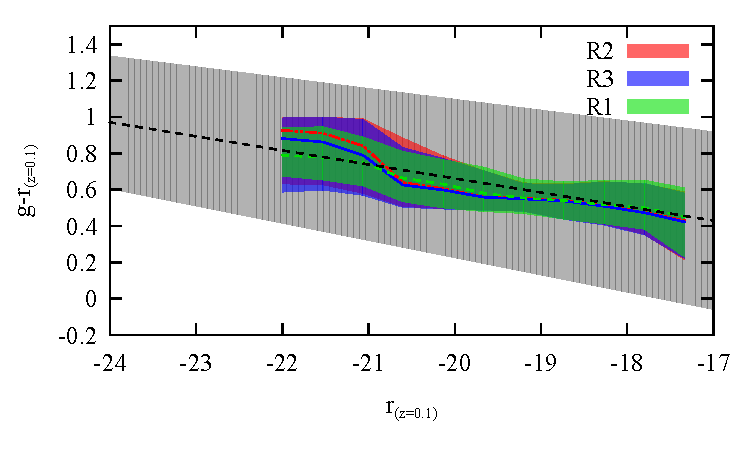
\includegraphics[scale=0.68]{figures/tests/Color_Mag.pdf}
\caption{ Color magnitud relation. Magnitudes were calculated without extintion. This is the reference simulation presented in table \ref{tab:runs}  as 
R1, R2 and R3. The shaded region correspond to a scatter of  $2\sigma$ from the work  of \citet{2012MNRAS.423.1583M}.\label{fig:CM-diagram}}
\end{figure}
We calculated the Tully-Fisher and Color-Magnitude relations for each of the models in Table \ref{tab:runs}.  
To build the Tully-Fisher relation, we proceded selecting the maximum velocity between the  bulge and disk components of disk galaxies, and defined
 disks as galaxies  with a bulge-to-total mass ratio $M_{\text{bulge}}/M_{\text{tot}}\le 0.3$. 

In Figure \ref{fig:T-F-diagram} are shown de scatters of the maximum velocity  between the first and thirth quartils  as a function of magnitude in
 the i-band without dust extintion of the data of the three benchmarks R1, R2 and R3 compared to the data of the SDSS \citep{2007AJ....134..945P}.
 It can be seen the resulting Tully-Fisher relations of each of the benchmarks reproduce accurately the one of the SDSS. In general none of the 
calculated Tully-Fisher relations of any of the simulated models deviate significantly from ones shown in \ref{fig:T-F-diagram}. We have also calculated the
 Color-Magnitude diagrams without dust extintion of the three mentioned benchmarks. In Figure \ref{fig:CM-diagram}, the scatter of the color between the 
first and thirth quartils and the medians as a function of the r-band reproduce accurately the estimated Color-Magnitude relation of the 
SDSS \citep{2012MNRAS.423.1583M}. Again, in general, all the other simulated models of the calculated medians does not deviate significantly from 
the estimations of the best fit of the mean of the SDSS and remains inside of the $3\sigma$ estimated deviation of the Color-Magnitude relation.


Besides, as we stated in Section \ref{sec:method:numericals}, we developed four experiments intended to study the changes in the stellar-to-dark matter ratio, 
gas-to-total mass ratio and bulge-to-total mass ratio of the simulated galaxies according to the variation in the different models of $\alpha_{\text{outflow}}$,
 $\epsilon_\star$, $\eta$ and  $M_{\text{satel.,gas}}\to$, as described in  Table \ref{tab:runs}. 

In Figure \ref{fig:properties-runs-compare} are presented the results of three of the above mentioned experiments. The three panels of the left row show
the results of the modification of the supernovae activity through four different values of $\alpha_{\text{outflow}}$ in the disk component of the 
simulated galaxies, the A-labeled models of Table \ref{tab:runs}; The three panels of the central row correspond to the E-labeled models,
where we modeled our halo population for six different values of $\epsilon_{\text{disk},\star}$; And, in the three right panels are the results of the D-labeled 
models, where it is modified the value of the $\eta$ parameter when $M_{\text{satel.,gas}}\to$ is settled to the disk component. 

The panels on top of
 Figure \ref{fig:properties-runs-compare} show the calculated medians of the stellar-to-dark matter ratio relations of each of the experiments, the central panels are the 
medians of the gas-to-total mass ratio as a funcion of the stellar mass and the ones at the bottom are medians of the bulge-to-total mass ratio as a function of the stellar mass. 
In the plot at the left on top, galaxies with a total stellar mass content below $3.2\times 10^{10}M_{\odot}$ shows a decrease in the amount of the stellar 
content as it is increased the rate of ejected mass by supernovae, and then, as it is expected, the amount of gas content is increased as can be seen 
at the left central plot. The morphology of the galaxies is affected as well. Shown at the bottom left panel of Figure \ref{fig:properties-runs-compare}, the
 net effect of increasing the $\alpha_{\text{disk, outflow}}$ parameter produces a decrease of the bulge-to-total mass ratio, so, it increases the amount 
of disk galaxies. Nevertheless the four values of the $\alpha_{\text{disk, outflow}}$ parameter keep the the gas-to-total mass ratio relations under good 
agreement with observations and the bulge-to-total mass ratio relations behaves as it is espected, only the values between $2.5$  and $3.0$ are the ones that
can enclose the stellar-to-halo mass relation. $2.5$  and $3.0$ are respectively  upper and lower limits of $\alpha_{\text{disk, outflow}}$ for the 
stellar-to-halo mass relation of \cite{2010ApJ...710..903M}.

In the top central panel of Figure \ref{fig:properties-runs-compare}, the stellar-to-halo mass relation show a trend related to the star 
formation in the disk component of galaxies. As  $\epsilon_{\text{disk},\star}$  increases the faint end of the stellar-to-halo mass relation tend to 
decrease while the bright end increases. It has to be remarked that while the stellar-to-halo mass relation changes, the calculated medians of the relation 
for the six different models remain almost fixed arround the peak of the relation at $1\times 10^{12}M_{\odot}$. In the central panel,  a low star formation
 rate in galaxies with a stellar mass lower than $3.2\times 10^{10}M_{\odot}$ increase the gas-to-total mass ratio.  In the  central bottom panel we can see 
the increase of the $\epsilon_{\text{disk},\star}$ clearly modifies the morphology of galaxies. A higher  $\epsilon_{\text{disk},\star}$ increases the disk 
component masses of the whole population of simulated galaxies and then the abundace of disk galaxies is increased.  Nevertheless the gas-to-total mass 
ratio relation keeps inside the observations for the different E-labeled models when is compared to the data provided in \cite{2003ApJS..149..289B} and 
\cite{2003ApJ...585L.117B}, the highest values of 
$\epsilon_{\text{disk},\star}$ are the ones that provide a relation  closer to the one of \cite{2010ApJ...710..903M}. The  three right panels of Figure 
\ref{fig:properties-runs-compare} show the results of the D-labeled models where it has been settled $M_{\text{satel.,gas}}\to$ to the disk component and
 simulated for different values of $\eta$. It was not found any correlation between the $\eta$ parameter and the calculated properties, not even when
 $M_{\text{satel.,gas}}\to$ was settled to the bulge in the B-labeled models.

\begin{figure*}
\centering
\begin{tabular}{c}
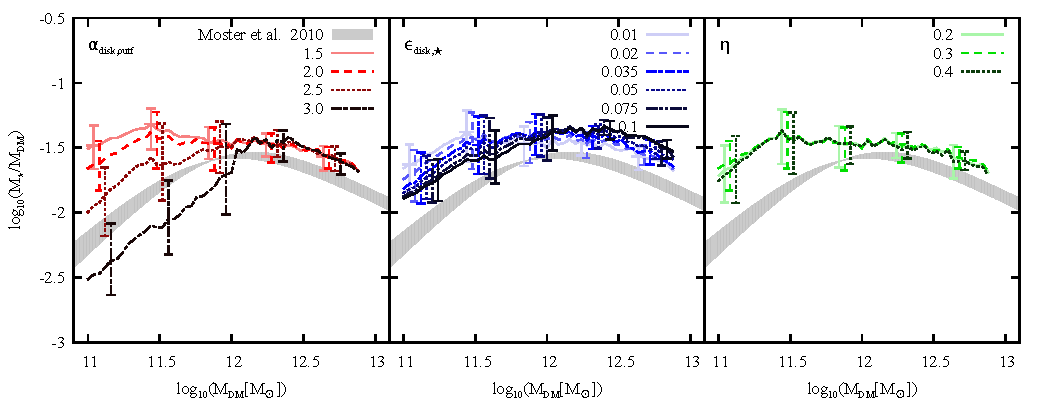
\includegraphics{figures/runs/run-v1-13-multiplot-star-frac.pdf} \\
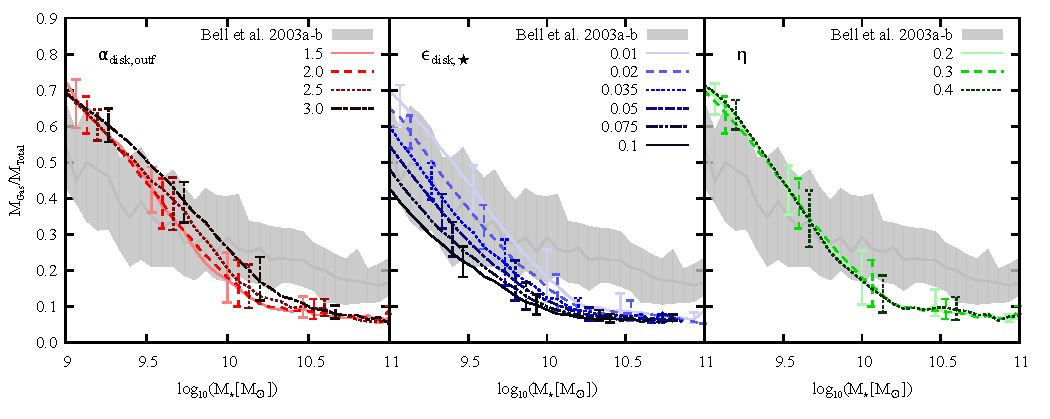
\includegraphics{figures/runs/run-v1-13-multiplot-gas-gfracscatter-quartils.pdf}\\
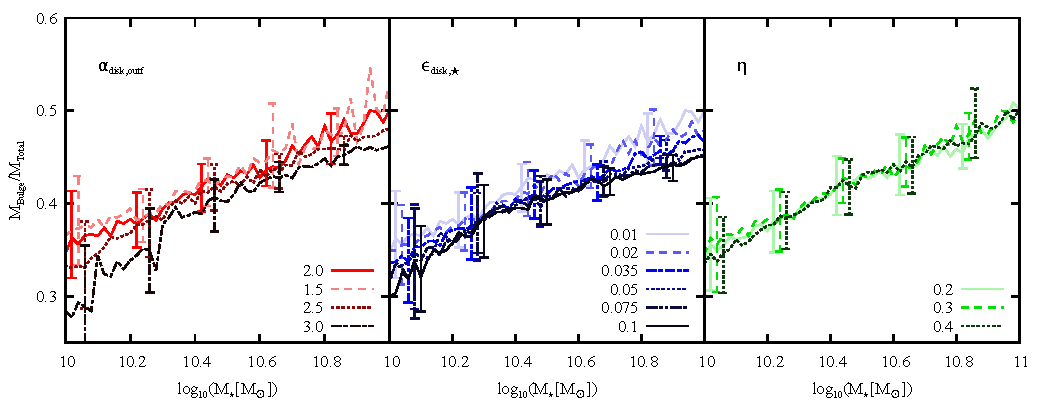
\includegraphics{figures/runs/run-v1-13-multiplot-bulge.pdf}
\end{tabular}
\caption{Top: Calculated medians of the stellar-to-halo mass relation compared against the relation of \citet{2010ApJ...710..903M} between the first and thirdth quartils. 
Central: Medians of the gas-to-total mass fraction as a  function of the stellar mass compared to \citet{2003ApJS..149..289B} and \citet{2003ApJ...585L.117B} between the 
first and thirdth quartils. Bottom: Medians of the  bulge-to-total mass fraction as a function of the stellar mass. The first
 row of the three plots correspond to the variation of the $\alpha_{\text{outflow}}$, the second to the variation  of $\epsilon_{\star}$ and the last to the 
variation of $\eta$ when the gas of the satellite goes to the disk of the galaxy. The error bars of each line correspond to the range of the data between the first and thirdth
quartils. 
\label{fig:properties-runs-compare}}
\end{figure*}

\subsection{Abundance of M31 and MW-type galaxies}
\begin{figure*}
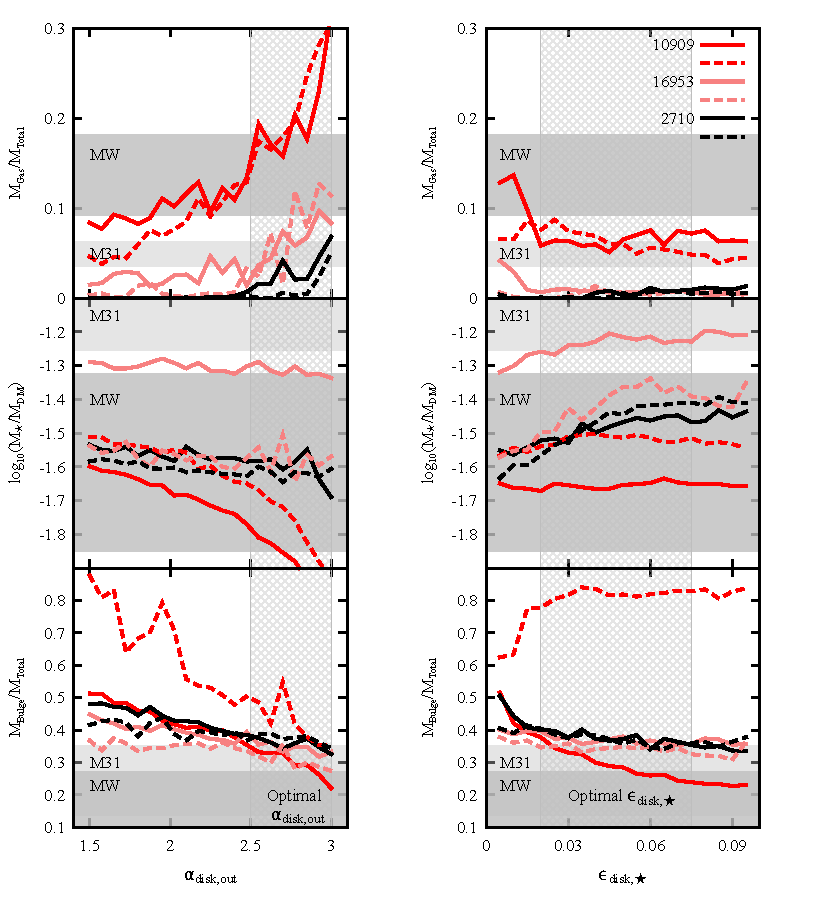
\includegraphics{figures/LG/LG-props-params-multi-v2.pdf}
\caption{Estimated medians of the modeled properties for the MW and M31 as a function of $\epsilon_{\star}$ on the right and $\alpha_{\text{outflow}}$ on the left.
 Top: Gas-to-total mass ratio. Central:Stellar mass-to-dark matter mass ratio relation.  Bottom: Bulge-to-total mass ratio relation. Horizontal shaded regions correspond to the observational
estimations of the MW and M31. The striped regions correspond to the values of the parameters that produce best agreement to the stellar-to-halo mass, gas-to-total mass relations and bulge
fraction.
%Horizontal line and dashed line are the MW and M31 observational references respectively in the gas and bulge
 %ratio relations.
\label{fig:properties-runs-LG}}
\end{figure*}

Now, we will analyse how changes the abundance of LG-type galaxies for the group of experiments defined in Table \ref{tab:runs}. To do that, 
we selected halos with a $z=0$ virial mass between  $11.5<\log_{10} M_{\text{DM}}/M_{\odot}<12.5$; calculated $N(\Delta\varepsilon)$ in ranges 
of $\Delta\varepsilon$ for the observed properties of the MW and M31 in Table \ref{tab:lg-observations}; and, study the $N(\Delta\varepsilon)$
 of the lowest values of $\Delta\varepsilon$ as a function of function of $\alpha_{outflow}$, $\epsilon_{\star}$, $\eta$ for the different models.
% The  normalized distribution functions $P(\log_{10}\chi)$ of the $\chi$ parameter shown in Figures \ref{fig:mw-hist-pdf} and \ref{fig:m31-hist-pdf}
% of  MW and M31-like galaxies respectively, were calculated  for the semi-analitycally simulated galaxies with halo mass in $11.0<\log_{10} M_{\text{DM}}<13.0$ 
% in four of the models of Table  \ref{tab:runs} taking into account the observational estimations in Table \ref{tab:lg-observations}. 
% The calculated distribution functions for the models shown in Figures \ref{fig:mw-hist-pdf} and \ref{fig:m31-hist-pdf} and all the other models show only small
%  variations while the medians tend to be around $\log_{10} \chi=0.5$ and keep almost the same scatter.
% \begin{figure}
% \centering
%  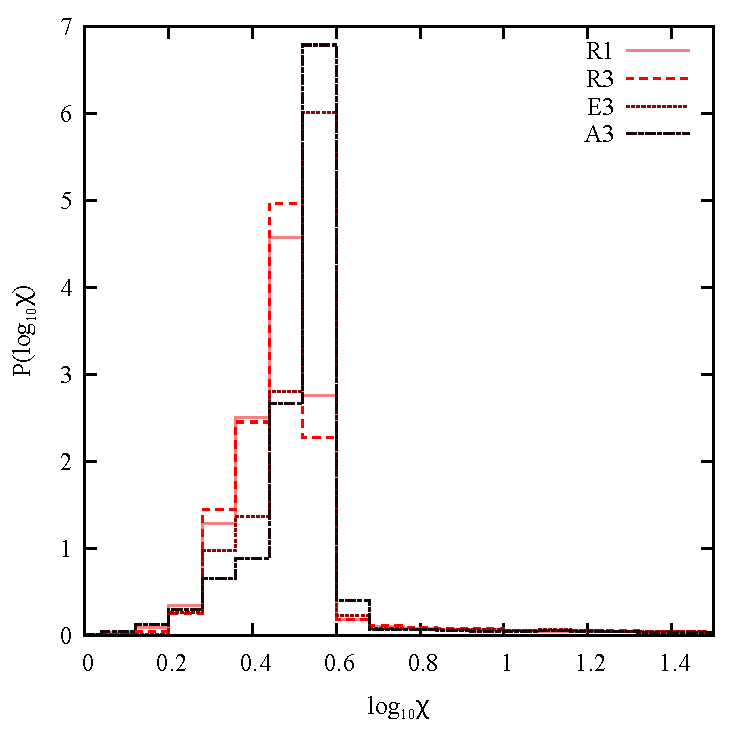
\includegraphics[scale=0.65]{figures/chi-histograms/run-v1-13-mw-chi-squared-no-halo-normal-histogram.pdf}
% \caption{ Distribution function of the parameter $\log_{10}\chi$ calculated for the  MW of four models of Table \ref{tab:runs}.\label{fig:mw-hist-pdf}}
% \end{figure}
% \begin{figure}
% \centering
%  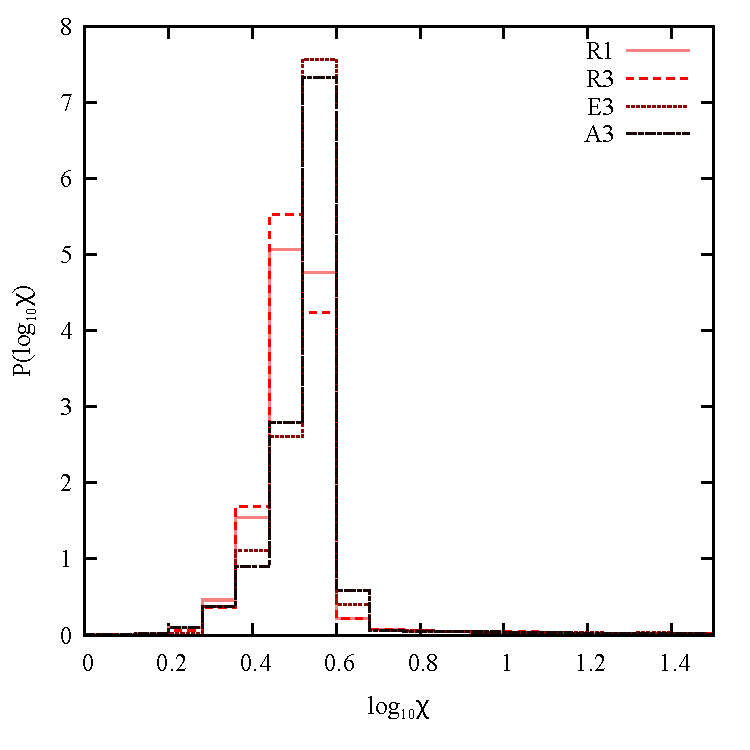
\includegraphics[scale=0.65]{figures/chi-histograms/run-v1-13-m31-chi-squared-no-halo-normal-histogram.pdf}
% \caption{ Distribution function of the parameter $\log_{10}\chi$ calculated for the  M31 of four models of Table \ref{tab:runs}. \label{fig:m31-hist-pdf}}
% \end{figure}
% We are specially interested in how the variation of the values of the parameters between the models of each experiment affect the abundace of MW and  
% M31-type galaxies. So, in order to find wether there is a correlation between any of the parameters of the experiments and the calculated distributions
%  of the models,  we studyed $P(\log_{10} \chi)$ as a 

In Figure \ref{fig:lg-chi-disk-outflow} are plotted the $N(\Delta\varepsilon)$ of the three lowest values of $\Delta\varepsilon$
for MW and M31-type galaxies as a function of $\alpha_{\text{outflow}}$ calculated  for the set of A-labeled models of Table  \ref{tab:runs}, where the 
value of $\alpha_{\text{outflow}}$ was increased from $1.5$ in steps of $0.5$  to $3.0$.  It can be observed that higher values of $\alpha_{\text{outflow}}$ 
increases the amount of LG-type galaxies but priviledges the increase of the abundace of MW-type galaxies more than that of M31-type galaxies. 


Nevertheless an increase of the value of $\alpha_{\text{outflow}}$ would produce a higher amount of LG-type galaxies, 
the overstate of the supernovae feedback activity produces a decrease of the stellar-to-halo mass relation for halos with 
$M_{\text{DM}}\le 1\times 10^{12}M_{\odot}$ as can be seen at the plot at the left on top of the Figure \ref{fig:properties-runs-compare}. We found that
 under the space parameter configuration of the simulated A-labeled models,  the proper values of $\alpha_{\text{outflow}}$ 
for modeling the supernovae feedback through  equation \ref{eq:supernovae} can only be  between $2.5 \lessapprox \alpha_{\text{outflow}} \lessapprox 3.0$,
 and, to increase the abundance of disk galaxies and then LG-type galaxies, should be choosen the highest values $\alpha_{\text{outflow}}$ below $3.0$.
\begin{figure}
\centering
 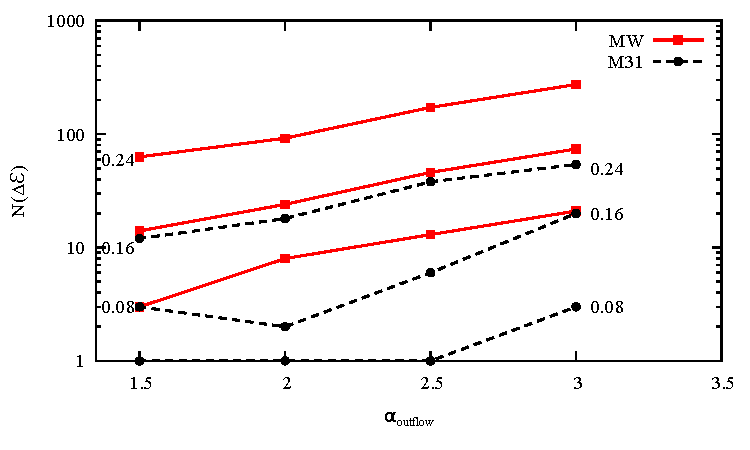
\includegraphics[scale=0.68]{figures/chi-parameters/chi-squared-disk-outflow-exp-v2.pdf}
\caption{$N(\Delta\varepsilon)$ as a function of $\alpha_{\text{outflow}}$. $N(\Delta\varepsilon)$ for the three lowest values of 
$\Delta\varepsilon=0.08,0.16,0.24$ as a consecuense of the variation of $\alpha_{\text{outflow}}$ parameter. \label{fig:lg-chi-disk-outflow}}
\end{figure}

We also made an analysis like the above with the $\epsilon_{\star}$ parameter for the E-labeled models. Figure \ref{fig:lg-chi-disk-star-eff} shows  
 the values of $N(\Delta\varepsilon)$ for the three lowest values of $\Delta\varepsilon$ calculated for LG-type galaxies as a function of $\epsilon_{\star}$.
 
Even though higher values of  $\epsilon_{\star}$ increases the abundace of disk galaxies, the increase  of the star  formation in the disk component of the 
sample of simulated galaxies does not favorate the formation of LG-type  galaxies, on the contrary, the decrease of the parameter favorates it.

The performed D-labeled simulations with different values of  $\eta$; intended to see wether this parameter affects the formation or LG-type galaxies or not,
showed no correlation between $\eta$ and $N(\Delta\varepsilon)$. As can be seen at the right plots of Figure \ref{fig:properties-runs-compare}, the shape of the
 simulated properties for our sample galaxies is not affected by the $\eta$ parameter. Nevertheless of the previous result, we found that the 
redirection of the gas of a satellite after  a minor merger to the disk instead of the bulge does favorate the searched situation, as it can be seen in Figure
 \ref{fig:lg-chi-gas-moves-to} where we compare $N(\Delta\varepsilon)$ of models R2 and R3 calculated for MW and M31-like galaxies.

\begin{figure}
\centering
 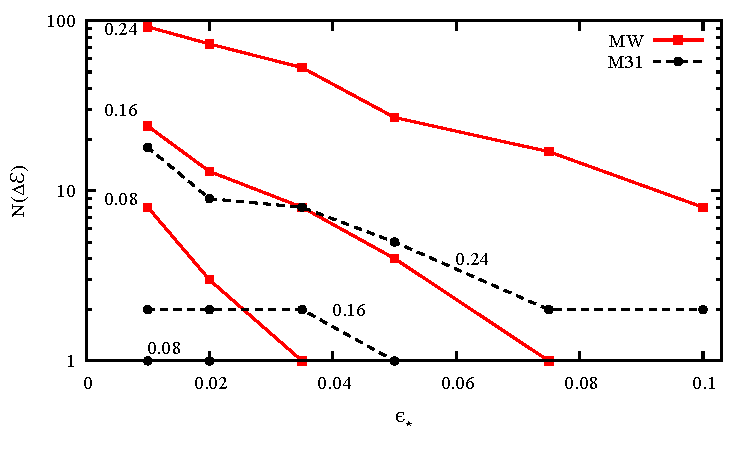
\includegraphics[scale=0.68]{figures/chi-parameters/chi-squared-star-form-eff-v2.pdf}dr
\caption{$N(\Delta\varepsilon)$ as a function of $\epsilon_{\star}$. $N(\Delta\varepsilon)$ for the three lowest values of $\Delta\varepsilon=0.08,0.16,0.24$ 
as a consecuenseof the variation of $\epsilon_{\star}$ parameter. \label{fig:lg-chi-disk-star-eff}}
\end{figure}


\begin{figure}
\centering
 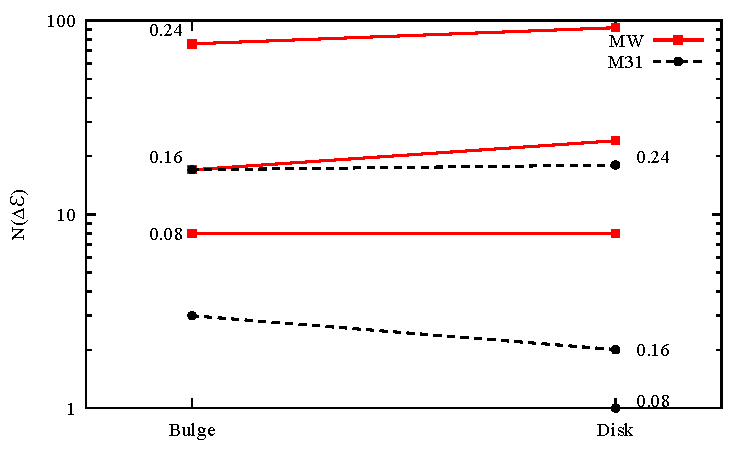
\includegraphics[scale=0.68]{figures/chi-parameters/chi-squared-merger-ratio-v2.pdf}
\caption{The values of $N(\Delta\varepsilon)$  for the three lowest values of $\Delta\varepsilon=0.08,0.16,0.24$ when the gas of a satellite after a merger goes to the 
disk and to de bulge. \label{fig:lg-chi-gas-moves-to}}
\end{figure}

\subsection{The MW and M31 candidates}
As described in section \label{sec:modeling-lg}, to study the LG candidates of the CLUES WMAP5 simulations we runned 20 models where we repeated over 100 times 
the estimation the properties in each of the models and the calculated the medians of each property. In Figure \ref{fig:properties-runs-LG} can be observed
the estimated medians for the stellar mass, gas fraction and bulge fraction as a function of the parameters $\epsilon_{\star}$ and $\alpha_{\text{outflow}}$.
It can be observed that each pair of LG corresponding to the same simulations have a similar behavior as the values of the parameters are changed.

\section{Conclusions and Discusion}
\label{sec:conclusions}

\section*{Acknowledgments}  

\bibliographystyle{mn2e}
\bibliography{references} 



\end{document}




